\chapter{Technical Decisions and Alternatives}

\section{Web Technologies}
\label{sec:web_technologies}

As we saw above, I implemented my prototype as a web application. The criteria for picking an implementation platform was that of accessibility to users and speed of development. Using that criteria I decided to make my prototype a web application as it's only entry barrier to users is that of a modern web browser. Web applications are a field that I have experience with and can quickly develop in. 

There are a few pitfalls to this approach that can be addressed through alternative implementations. Because my application is primarily a prototype for illustrating effective exploration features, the issue of scale is not one that was addressed. If a web application was used for enterprise size provenance files the application may soon run out of resources required to render it.

An alternative to a web application would be to write the prototye in an OS independent language such as Java or Python; this would allow wide accessibility and more fine grained control of machine resources. However if an OS level language was chosen issues could later occur in presenting provenance on mobile devices as there aren't may languages that run on both desktop and mobile devices without heavy modifications. Consequently if an OS dependant languages such as Apple's swift of Microsoft's C\# was used features and code would have to be replicated for the different OS languages (assuming that OS independent accessibility is an important criteria).

The standard technology for data visualisation in a browser is the D3.js\footnote{D3: Data Driven Documents \url{https://d3js.org/}} JavaScript library. However as mentioned earlier, I used Cytoscape.js to implement my interface because it's specifically focused on graph theory and has a lot of inbuilt functions such as rendering and events. If this application was to be re-written using D3, a lot more of the fundemental functions of Cytoscape would have to be written from scratch, however it would allow for more fine-grained control of the appplication, this could particularly be useful when dealing with exceptionally large files.

\section{Client Side Processing}
\label{sec:client_side_processing}

As we saw before, the visualiser loads the file on the client side and renders it locally. When first outlining features of the application I wanted it to be primarily stand alone. This means that even though it can run of a web server, you could just as easily run it locally on your computer with minimal effort because all proccessing and computation is done client side. 

However server side computation may be a useful feature for the future, a server with higher computational power and resources may be able to find and analyze interesting details about the file. The naive approach to accomplishing this would to have the file uploaded to the server, analytics run on the provenance and then results downloaded back to the client. An alternative approach however would to have the client select only the neccessary sectinos required for analysis and send those to the server. The client could then render the provenance locally whilst results where computed and finally render the results onto the already drawn graph. This allows the user to begin exploring the graph immediately as well as minimising the amount of bandwidth used by the application.

\section{Node Clustering}
One of the earliest features we discussed when outlining how to visualise provenance was the ability to cluster and create composite nodes. The feature of allowing multiple nodes to be grouped into a single representative node has two main purposes. Firstly it allows simplification of the graph, this is useful when showing someone a speficit section of the graph as well as easier conceptual understanding when exploring. Secondly it is useful when securing graphs and composite nodes can be used to obviscate information.

Cytoscape.js doesn't have a group feature, so it was required to write one from scratch. The key test for this function is that grouping and ungrouping nodes is undestructive: if a series of nodes are grouped and then ungrouped the resulting graph must be isomorphic to the original.

\begin{figure}[h]
  \centering
  \begin{subfigure}[t]{0.5\textwidth}
    \includegraphics[width=\textwidth]{ungrouped}
    \caption{Graph with no composite nodes}
  \end{subfigure}
  ~
  \begin{subfigure}[t]{0.5\textwidth}
    \includegraphics[width=\textwidth]{grouped}
    \caption{Same graph with a composite node}
  \end{subfigure}
  \caption{An example of a composite node containing the \textit{Tweets}, \textit{X-tweets-1}, \textit{X-tweets-2} and \textit{X-tweets-3} nodes.}
\end{figure}

Nodes removed from Cytoscape.js can be `restored' into their original position, unfortunately any edged associated with the node are permenately destroyed. It is neccessary then to store the edges as a data field in the composite node so that when restoring nodes, edges can also be recreated. 

\begin{figure}[h]
  \centering
  \begin{lstlisting}
 // Create composite node and fields for original edges and nodes.
 Create new CompositeNode 
 CompositeNode.originalEdges = All edges in neighbourhood of selected nodes
 CompositeNode.originalNodes = All nodes that where grouped

 // Create new edges from external nodes to CompositeNode
 for each edge in neighbourhood {
  if (edge != internal to group)  {
    Create new Edge({from: externalNode, to:compositeNode})
  }
 }

 // Remove original nodes
 Remove selected nodes
 \end{lstlisting}
 \caption{Pseudocode: Creaing a composite node}
\end{figure}

However the above code only works in a limited scenario: ungrouping nodes in the oposite order of creation. For example if you created comisite nodes $A$, $B$, $C$ (cronologically and all with neighbouring edges) you would have to ungroup them in the following order: $C$, $B$, $A$. If you where to for example ungroup node $A$ first, when ungrouping $C$ it would try to restore edges to the now non-existent $A$ compsosite node. In order to tackle this I created the group manager class.

The Group Manager class is the primary way of keeping track of nodes that are hidden inside composite nodes. It contains a tree data structure that references all the groups as well as their child nodes/groups. Now when ungrouping nodes this class is called and the parent group of the child node requested, then a new temporary edge is created to the composite node and the original edge stored in a \textit{hanging edges} object until it can be restored. Every time a group is created or destroyed the \textit{hanging edges} object is queried to see if any originl edges can be recreated.

\subsection{Clustering example: Without \textit{Group Manager} or \textit{Hanging Edges}}

Below is an example of issues that occur when trying to ungroup nodes in the incorrect order without the supporting classes \textit{Group Manager} and the hanging edges object. As seen in the final step, all the edges are lost, a less than ideal situation and in failure of the primary test of having an isomorphic graph after grouping and ungrouping nodes.

\begin{figure}[H]

  \begin{subfigure}[t]{0.5\textwidth}
    \centering
    \begin{tikzpicture}
      \node[main node] (A1) {A1};
      \node[main node] (A2) [right of=A1] {A2};
      \node[main node] (B1) [below of=A1] {B1};
      \node[main node] (B2) [below of=A2] {B2};
      \path (A1) edge node[left] {used} (B1);
      \path (A2) edge node[left] {used} (B2);
    \end{tikzpicture}
    \caption{Nodes $A1$ and $B1$ are linked, nodes $A2$ and $B2$ are linked.}
  \end{subfigure}
  ~
  \begin{subfigure}[t]{0.5\textwidth}
    \centering
    \begin{tikzpicture}
      \node[main node, group] (CA) {CA};
      \node[main node] (B1) [below left of=CA] {B1};
      \node[main node] (B2) [below right of=CA] {B2};
      \path (CA) edge node[left] {used} (B1);
      \path (CA) edge node[right] {used} (B2);
    \end{tikzpicture}
    \caption{Group nodes $A1$ and $A2$ into composite node $CA$. Stored inside the composite node is the original edges from $A1\rightarrow B1$ and $A2\rightarrow B2$.}
  \end{subfigure}
  \begin{subfigure}[t]{0.5\textwidth}
    \centering
    \begin{tikzpicture}
      \node[main node, group] (CA) {CA};
      \node[main node, group] (CB) [below of=CA] {CB};
      \path (CA) edge node[right] {used} (CB);
    \end{tikzpicture}
    \caption{Group nodes $B1$ and $B2$ insto composite nodes $CB$. Stored inside the composite node $CB$ is the edges from $CA\rightarrow B1$ and $CA\rightarrow B2$.}
  \end{subfigure}
  ~
  \begin{subfigure}[t]{0.5\textwidth}
    \centering
    \begin{tikzpicture}
      \node[main node, group] (CB) {CB};
      \node[main node] (A1) [above left of=CB] {A1};
      \node[main node] (A2) [above right of=CB] {A2};
    \end{tikzpicture}
    \caption{Ungroup $CA$. It will try to create adges between $A1\rightarrow B1$ and $A2\rightarrow B2$, because $B1$ and $B2$ are currently in a group, the new edges will fail and not be rendered.}
  \end{subfigure}
  \begin{subfigure}[t]{0.5\textwidth}
    \centering
    \begin{tikzpicture}
      \node[main node] (A1) {A1};
      \node[main node] (A2) [right of=A1] {A2};
      \node[main node] (B1) [below of=A1] {B1};
      \node[main node] (B2) [below of=A2] {B2};
    \end{tikzpicture}
    \caption{Ungroup $CB$. Edges between $CA\rightarrow B1$ and $CA\rightarrow B2$ will try to be restored but because there's no $CA$ in the graph these will fail.}
  \end{subfigure}
\end{figure}

\subsection{Clustering example: Working isomorphic grouping with helping classes.}
As mentioned previously we want to complete the test of having an isomorphic graph after grouping and ungrouping nodes. To do this we use both a class \textit{GroupManager} and an array \textit{HangingEdges}. The \textit{GroupManager} stores a tree to monitor groups and nodes inside them, it also has some helper functions for adding groups and finding the upmost group of a certain node. The \textit{HangingEdges} array is simply a list of edges that couldn't be restored because one or more of the connected nodes where missing.

In the figure below the left hand side shows the state of the graph, whilst the right hand side shows the \textit{GroupManager} as well as the content of \textit{HangingEdges}.

\begin{figure}[H]

  \begin{subfigure}[t]{0.5\textwidth}
    \centering
    \renewcommand\thesubfigure{A1}
    \begin{tikzpicture}
      \node[main node] (A1) {A1};
      \node[main node] (A2) [right of=A1] {A2};
      \node[main node] (B1) [below = 1cm of A1] {B1};
      \node[main node] (B2) [below = 1cm of A2] {B2};
      \path (A1) edge node[left] {used} (B1);
      \path (A2) edge node[left] {used} (B2);
    \end{tikzpicture}
    \caption{Nodes $A1$ and $B1$ are linked, nodes $A2$ and $B2$ are linked.}
  \end{subfigure}
  ~
  \begin{subfigure}[t]{0.5\textwidth}
    \renewcommand\thesubfigure{A2}
    \centering
    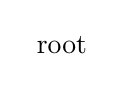
\begin{tikzpicture}
      \node[] (root) {root};
    \end{tikzpicture}
    \caption{The GMTree (Group Manager Tree) is currently empty and Hangingedges = [].}
  \end{subfigure}
  \begin{subfigure}[t]{0.5\textwidth}
    \centering
    \renewcommand\thesubfigure{B1}
    \begin{tikzpicture}
      \node[main node, group] (CA) {CA};
      \node[main node] (B1) [below left of=CA] {B1};
      \node[main node] (B2) [below right of=CA] {B2};
      \path (CA) edge node[left] {used} (B1);
      \path (CA) edge node[right] {used} (B2);
    \end{tikzpicture}
    \caption{Group nodes $A1$ and $A2$ into composite node $CA$. Stored inside the composite node is the original edges from $A1\rightarrow B1$ and $A2\rightarrow B2$.}
  \end{subfigure}
  ~
  \begin{subfigure}[t]{0.5\textwidth}
    \centering
    \renewcommand\thesubfigure{B2}
    \begin{tikzpicture}
      \node[] (root) {root};
      \node[below = 1cm of root] (CA) {CA};
      \node[below right = 1cm of CA] (A1) {A1};
      \node[below left = 1cm of CA] (A2) {A2};
      \path (root) edge (CA);
      \path (CA) edge (A1);
      \path (CA) edge (A2);
    \end{tikzpicture}
    \caption{The GMTree holds information about $CA$, $A1$ and $A2$. Hangingedges = [].}
  \end{subfigure}

  \begin{subfigure}[t]{0.5\textwidth}
    \renewcommand\thesubfigure{C1}
    \centering
    \begin{tikzpicture}
      \node[main node, group] (CA) {CA};
      \node[main node, group] (CB) [below of=CA] {CB};
      \path (CA) edge node[right] {used} (CB);
    \end{tikzpicture}
    \caption{Group nodes $B1$ and $B2$ insto composite nodes $CB$. Stored inside the composite node $CB$ is the edges from $CA\rightarrow B1$ and $CA\rightarrow B2$.}
  \end{subfigure}
  ~
  \begin{subfigure}[t]{0.5\textwidth}
    \centering
    \renewcommand\thesubfigure{C2}
    \begin{tikzpicture}
      \node[] (root) {root};
      \node[below right = 1cm of root] (CA) {CA};
      \node[below right = 0.5cm of CA] (A1) {A1};
      \node[below left = 0.5cm of CA] (A2) {A2};

      \node[below left = 1cm of root] (CB) {CB};
      \node[below right = 0.5cm of CB] (B1) {B1};
      \node[below left = 0.5cm of CB] (B2) {B2};
      \path (root) edge (CA);
      \path (CA) edge (A1);
      \path (CA) edge (A2);
      \path (root) edge (CB);
      \path (CB) edge (B1);
      \path (CB) edge (B2);
    \end{tikzpicture}
    \caption{The GMTree holds information about all nodes. Hangingedges = [].}
  \end{subfigure}

  \begin{subfigure}[t]{0.5\textwidth}
    \centering
    \renewcommand\thesubfigure{D1}
    \begin{tikzpicture}
      \node[main node, group] (CB) {CB};
      \node[main node] (A1) [above left of=CB] {A1};
      \node[main node] (A2) [above right of=CB] {A2};
      \path (A1) edge node[left] {used} (CB);
      \path (A2) edge node[right] {used} (CB);
    \end{tikzpicture}
    \caption{CA is ungrouped and removed from the group manager tree. The original edges $A1\rightarrow B1$ and $A2\rightarrow B2$ can't be restored because B1 and B2 are currently hidden inside CB, these edges are stored in the hanging edges object. New edges are created by finding the upmost node using the group manager tree.}
  \end{subfigure}
  ~
  \begin{subfigure}[t]{0.5\textwidth}
    \centering
    \renewcommand\thesubfigure{D2}
    \begin{tikzpicture}
      \node[] (root) {root};
      \node[below = 1cm of root] (CB) {CB};
      \node[below right = 0.5cm of CB] (B1) {B1};
      \node[below left = 0.5cm of CB] (B2) {B2};
      \path (root) edge (CB);
      \path (CB) edge (B1);
      \path (CB) edge (B2);
    \end{tikzpicture}
    \caption{The GMTree holds information about $B$ nodes. $A$ nodes have been remove because they've been ungrouped. Hangingedges = [$A1\rightarrow B1$, $A2\rightarrow B2$].}
  \end{subfigure}

  \begin{subfigure}[t]{0.5\textwidth}
    \centering
    \renewcommand\thesubfigure{E1}
    \begin{tikzpicture}
      \node[main node] (A1) {A1};
      \node[main node] (A2) [right of = A1] {A2};
      \node[main node] (B1) [below = 1cm of A1] {B1};
      \node[main node] (B2) [below = 1cm of A2] {B2};
      \path (A1) edge node[left] {used} (B1);
      \path (A2) edge node[left] {used} (B2);
    \end{tikzpicture}
    \caption{CB is ungrouped and removed from the group manager tree. An attempt to restore hanging edges is made and both $A1\rightarrow B1$ and $A2\rightarrow B2$ are restored.}
  \end{subfigure}
  ~
  \begin{subfigure}[t]{0.5\textwidth}
    \centering
    \renewcommand\thesubfigure{E2}
    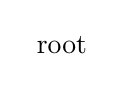
\begin{tikzpicture}
      \node[] (root) {root};
    \end{tikzpicture}
    \caption{The GMTree is empty because there's no groups. Hangingedges = [] because the previously stored edges have been restored.}
  \end{subfigure}
\end{figure}
